\subsection{Combustor [Thomas Satterly]}
The chosen combustor was a gaseous ethylene fueled RDE. The sizing of the combustion chamber was based off of the Bykovskii (REF XXX) guidelines and experimentally observed cell sizes for gaseous ethylene (REF XXX). Chapman-Jouget detonation parameters were calculated using the NASA CEA program, and the RDE performance was analyzed using the model proposed by Stechmann (REF XXX). The mass flow rate, minimum pressure, and minimum temperature were varied and the design iterated, along with the inlet, isolator, and compression duct, until a reasonable flow path was found with acceptable performance. 
    From experimental data collected by Bull, et. al., (REF XXX), the approximate cell size of an ethylene-air mixture at 195 kPa is approximately 12.6 mm. From the guidelines given by Bykovskii in equations EQ through EQ, the bounds on the RDE size can be calculated.

< Bykovskii equations here>

    From these guidelines, the RDE outer diameter was chosen at 0.2035 m with an inner diameter of 0.16 m and a total length of 0.254 m. A CAD model of the combustor can be seen in figure \ref{fig:combustorIsoView}.

\begin{figure}[H]
\begin{center}
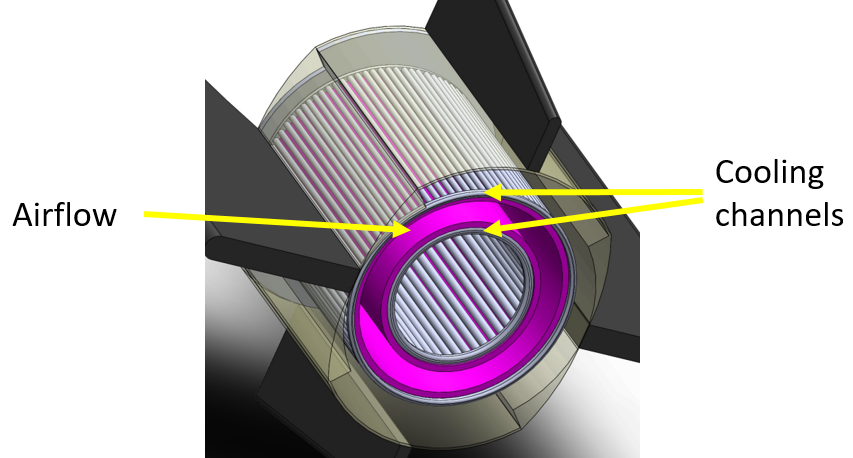
\includegraphics[width=0.7\textwidth]{combustorIsoView}
\caption{Combustor Geometry}
\label{fig:combustorIsoView}
\end{center}
\end{figure}

    Using the Stechmann model, the RDE’s performance was analyzed across the flight conditions the vehicle would experience. During acceleration, an equivalence ratio of 1 was chosen to capitalize on performance while avoiding extreme temperatures. During cruise, the equivalence ratio was reduced to 0.58 in order to produce enough thrust for steady level flight. The performance characteristics of the RDE is shown in table EQ. Detailed plots of the predicted flow parameters between detonation fronts can be found in the appendix.

\begin{center}
\begin{tabular}{l c c}
& Acceleration & Cruise \\
\hline
Isp(s) & 2131-2219 & 2080 \\
Thrust (N) & 3076-1963 & 1007.19 \\
Air Mass Flog (kg/s) & 3.868-3.346 & 3.346 \\
Fuel Mass Flow (kg/s) & 0.262 - 0.227 & 0.131 \\
Cf & 1.61 - 1.67 & 1.664 \\
C* (m/s) & 1444 & 1326 \\
Eq. Ratio & 1 & 0.58 \\
CJ Pressure Ratio & 5.327 - 5.11 & 4.25 \\
CJ Temperature Ratio & 2.93 - 2.84 & 2.54 \\
Combustor Mach & 1.5 - 2.14 & 2.14 \\
Entrance Pressure (kPa) & 250 - 195 & 195
\end{tabular}
\end{center}

    A major assumption made in this model is the ability for an RDE to be able to deep throttle from an equivalence ratio of 1 down to 0.58. Such a shift will affect the cell size and impose transients during throttling, of which neither effect has been studied in detail and remains an important question for the true capability of an RDE. 
